\documentclass{homework}
\usepackage{pgfplots}
\usepackage{subfig}
\usepackage{float}

\author{Juniper Huang \ \ \ \ \ \ \ \ \ \ \ \ \ \ \ \ \ \ \ \ \ \ \ \ \ \ \ \ \ \ \ \ \ \ \ \ \ \ \ \ \ \ \ \ \ \ \ \ \ \ \ \ \ \ \ \ \ \ \ \ \ \ \ \ \ \ \ \ \ \ \ \ \ \ \ \ \ \ \ \ \ \ \ \ 662115954}
\class{CSCI 6100 \ \ \ \ \ \ \ \ \ \ \ \ \ \ \ \ \ \ \ \ \ \ \ \ \ \ \ \ \ \ \ \ \ \ \ \ \ \ \ \ \ \ \ \ \ \ \ \ \ \ \ \ \ \ \ \ \ \ \ \ \ \ \ \ \ \ \ \ \ \ \ \ \ \ \ \ \ \ \ \ \ \ \ \ \ \ \ \ \ \today}
\title{Homework 7}

\graphicspath{{./media/}}
\begin{document}
\maketitle
\section{Classifying Handwritten Digits}

\begin{itemize}
    \item[a and b.] Plot separator and calculate \(E_{in}\) and \(E_{test}\)
    \begin{itemize}
        \item[i.] Linear Regression and Pocket Algorithm
        \begin{figure}[h]
            \centering
            \subfloat{{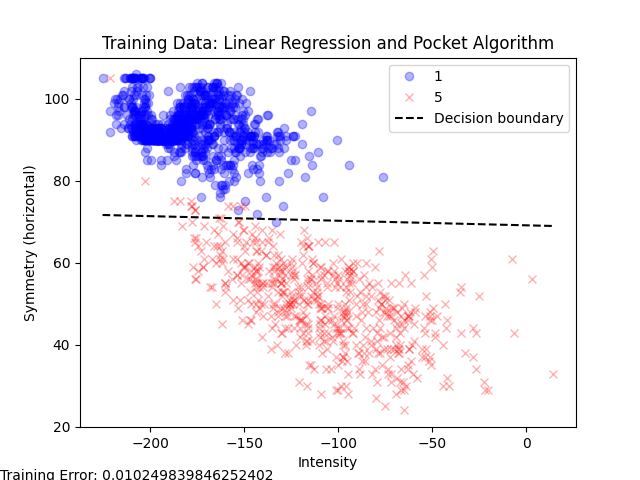
\includegraphics[width=8cm]{images/Part A/LinRegPocketTrain.png} }}%
            \qquad
            \subfloat{{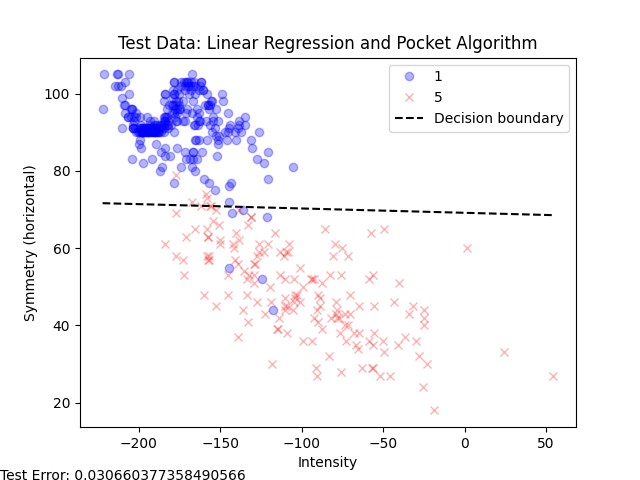
\includegraphics[width=8cm]{images/Part A/LinRegPocketTest.png} }}%
        \end{figure}

        \item[ii.] Linear Regression and Gradient Descent
        \begin{figure}[h]
            \centering
            \subfloat{{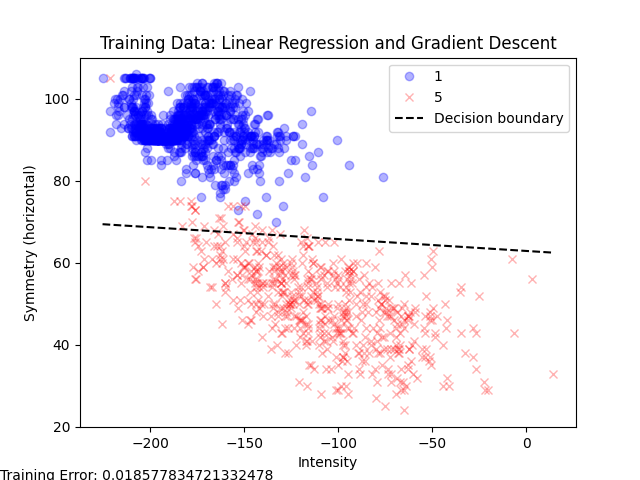
\includegraphics[width=8cm]{images/Part A/LinRegGradientTrain.png} }}%
            \qquad
            \subfloat{{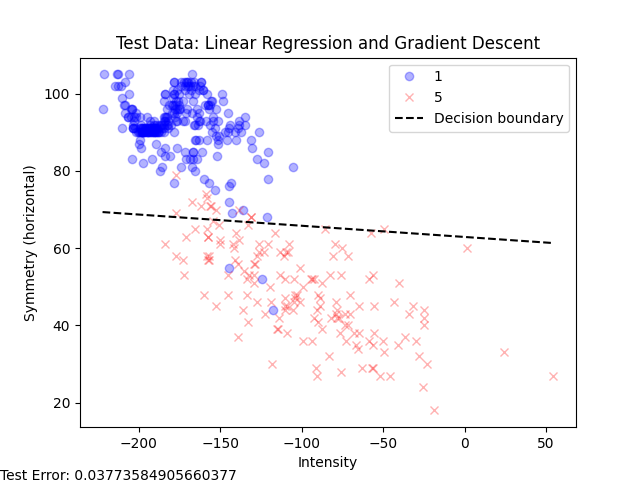
\includegraphics[width=8cm]{images/Part A/LinRegGradientTest.png} }}%
        \end{figure}
        
        \item[iii.] Linear Regression and Stochastic Gradient Descent
        \begin{figure}[H]
            \centering
            \subfloat{{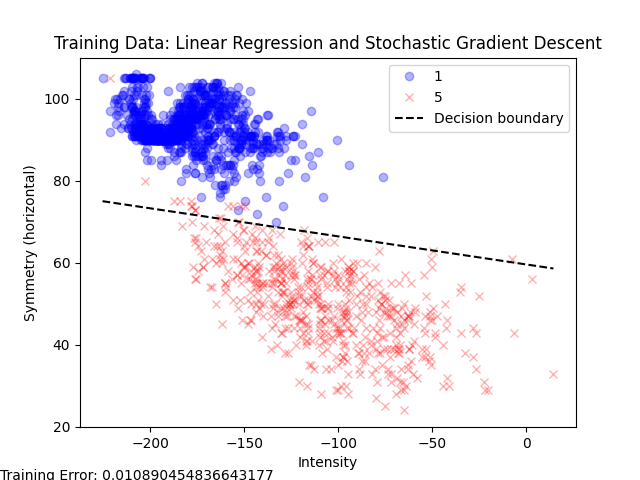
\includegraphics[width=8cm]{images/Part A/LinRegStochasticTrain.png} }}%
            \qquad
            \subfloat{{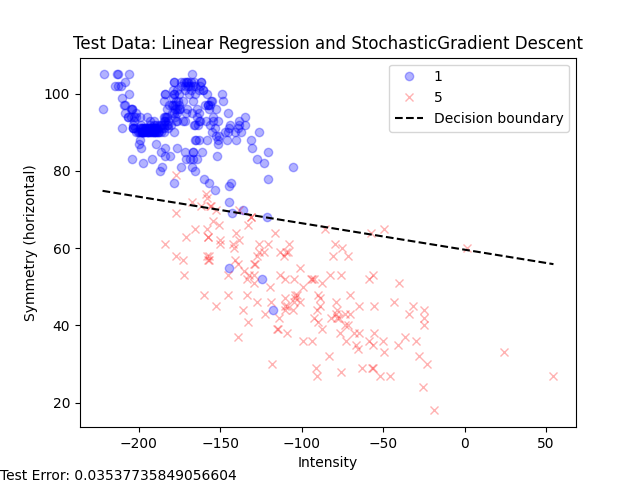
\includegraphics[width=8cm]{images/Part A/LinRegStochasticTest.png} }}%
        \end{figure}
        
        \item[iv.] Linear Programming
        \begin{figure}[H]
            \centering
            \subfloat{{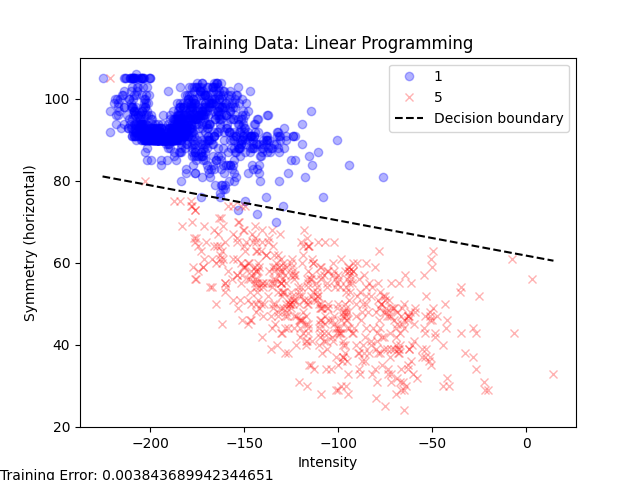
\includegraphics[width=8cm]{images/Part A/LinProgTrain.png} }}%
            \qquad
            \subfloat{{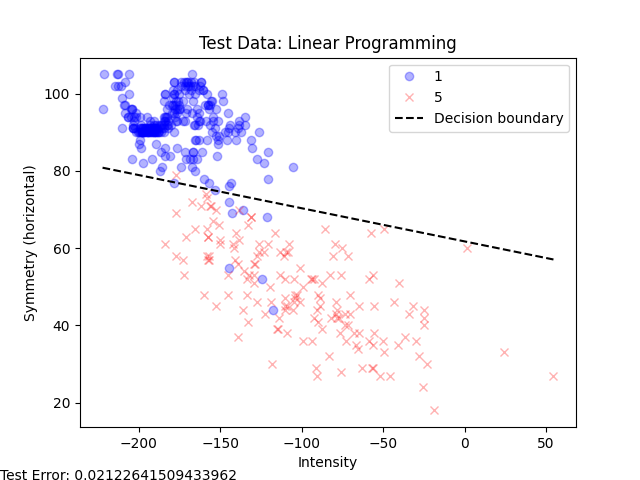
\includegraphics[width=8cm]{images/Part A/LinProgTest.png} }}%
        \end{figure}
    \end{itemize}
    
    \item[c.] Linear programming had the smallest \(E_{in} = .0038\). Using the Hoeffding bound equation, the upper bound of \(E_{out} = .0381\). 
    
    \item[d.]Linear programming had the smallest \(E_{test} = .0212\). Using the Hoeffding bound equation, the upper bound of \(E_{out} = .0871\).
    
    \item[e.] 3rd order polynomial transform
    \begin{itemize}
        \item[i.] Linear Regression and Pocket Algorithm
        \begin{figure}[H]
            \centering
            \subfloat{{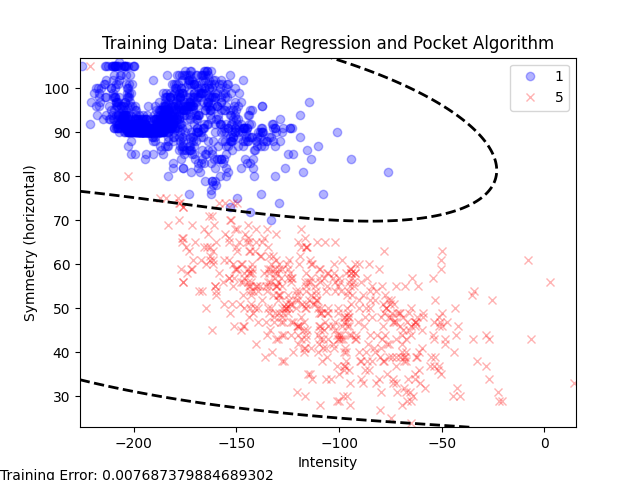
\includegraphics[width=8cm]{images/Part E/LinRegPocketTrain2.png} }}%
            \qquad
            \subfloat{{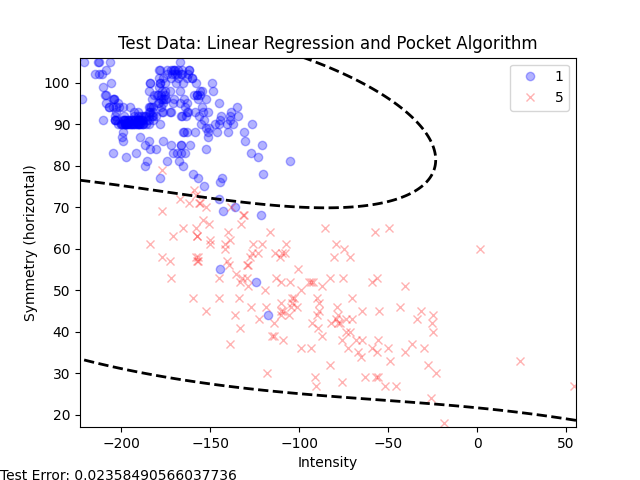
\includegraphics[width=8cm]{images/Part E/LinRegPocketTest2.png} }}%
        \end{figure}

        \item[ii.] Linear Regression and Gradient Descent
        \begin{figure}[H]
            \centering
            \subfloat{{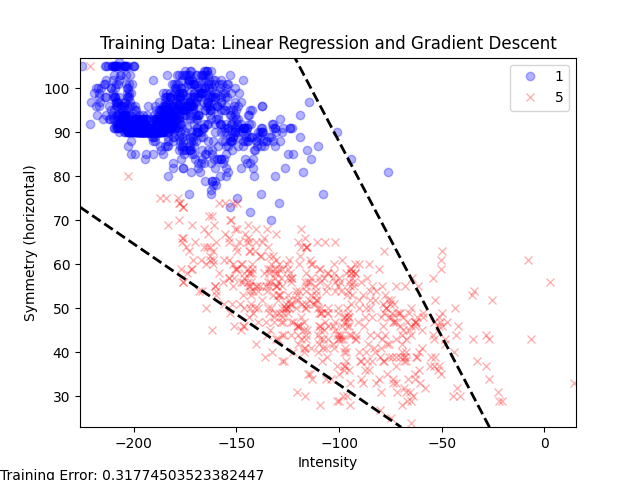
\includegraphics[width=8cm]{images/Part E/LinRegGradientTrain2.png} }}%
            \qquad
            \subfloat{{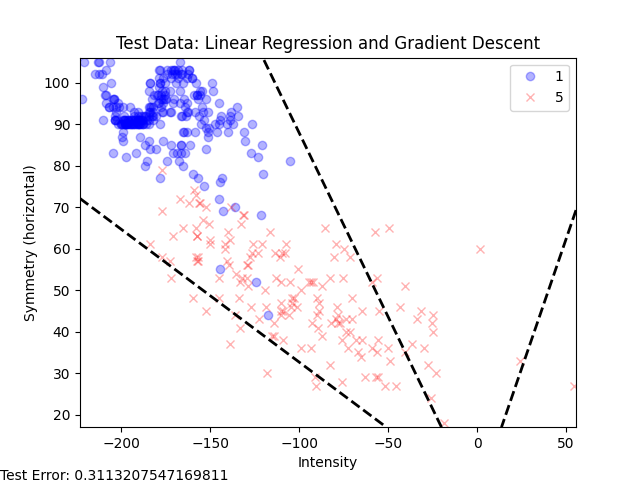
\includegraphics[width=8cm]{images/Part E/LinRegGradientTest2.png} }}%
        \end{figure}
        
        \item[iii.] Linear Regression and Stochastic Gradient Descent
        \begin{figure}[H]
            \centering
            \subfloat{{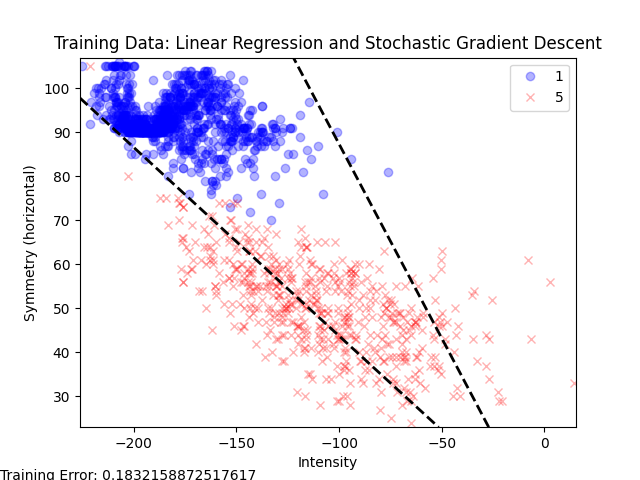
\includegraphics[width=8cm]{images/Part E/LinRegStochasticTrain2.png} }}%
            \qquad
            \subfloat{{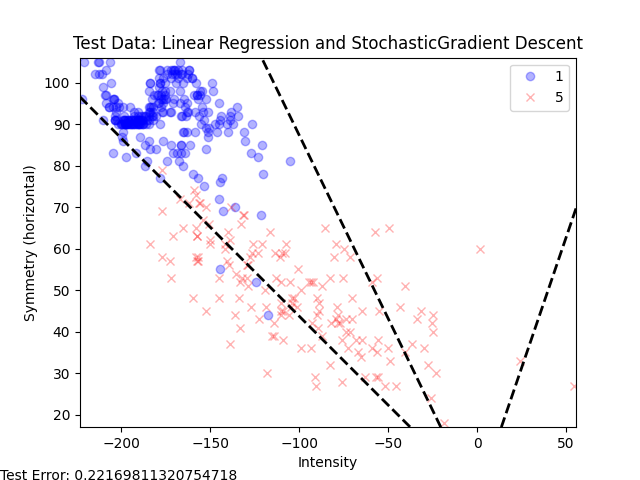
\includegraphics[width=8cm]{images/Part E/LinRegStochasticTest2.png} }}%
        \end{figure}
        
        \item[iv.] Linear Programming
        \begin{figure}[H]
            \centering
            \subfloat{{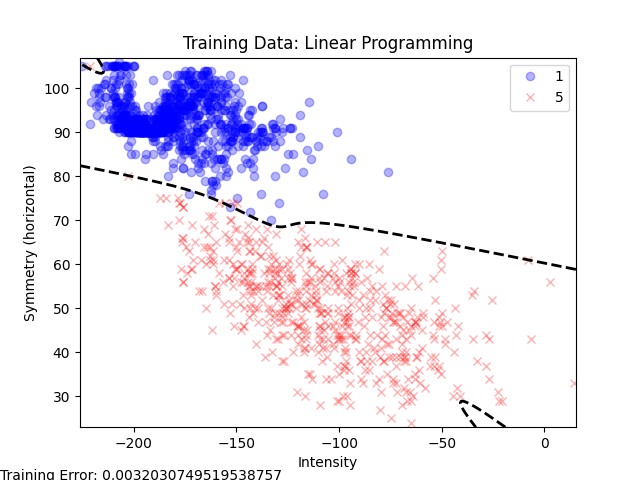
\includegraphics[width=8cm]{images/Part E/LinProgTrain2.png} }}%
            \qquad
            \subfloat{{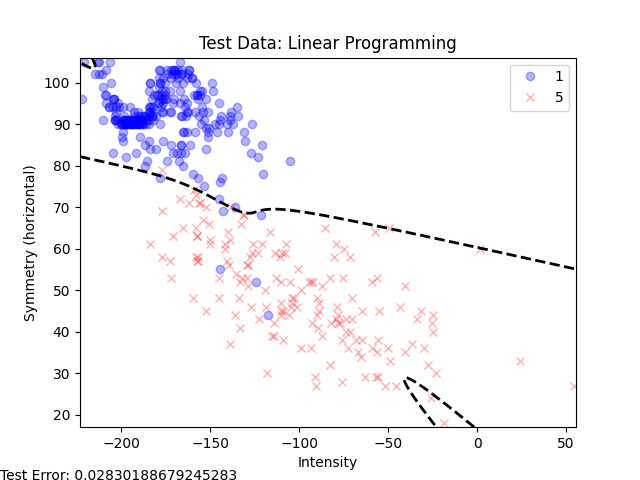
\includegraphics[width=8cm]{images/Part E/LinProgTest2.png} }}%
        \end{figure}
    \end{itemize}
    Linear programming had the smallest \(E_{in} = .0032\). Using the Hoeffding bound equation, the upper bound of \(E_{out} = .0376\).\\
    Linear programming had the smallest \(E_{test} = .0283\). Using the Hoeffding bound equation, the upper bound of \(E_{out} = .0942\).
    \item[f.] I would use the linear model without the polynomial transform. It is simpler and linear programming without transformation has the smallest \(E_{in}\) and \(E_{out}\). 
    
\end{itemize}

\section{Gradient Descent}
\begin{itemize}
    \item[a. ] When \(\eta =.01\), the function value quickly decreases and then bottoms out. This is in stark opposition to \(\eta = .1\) where the value increases and decreases randomly, meaning the step is too big. 

    \begin{figure}[H]
            \centering
            \subfloat{{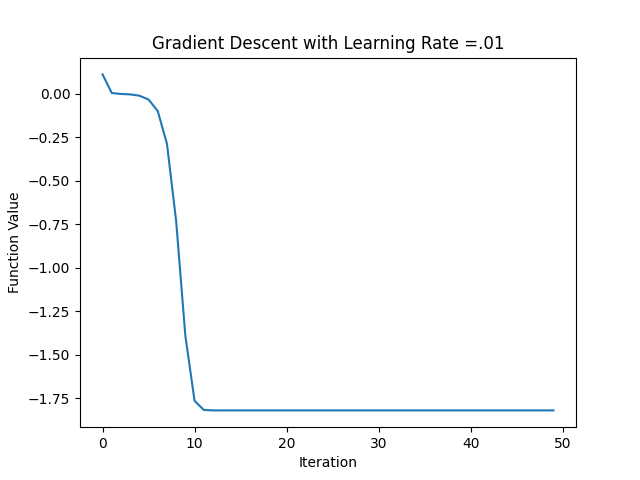
\includegraphics[width=8cm]{images/Question2/SmallerRate.png} }}%
            \qquad
            \subfloat{{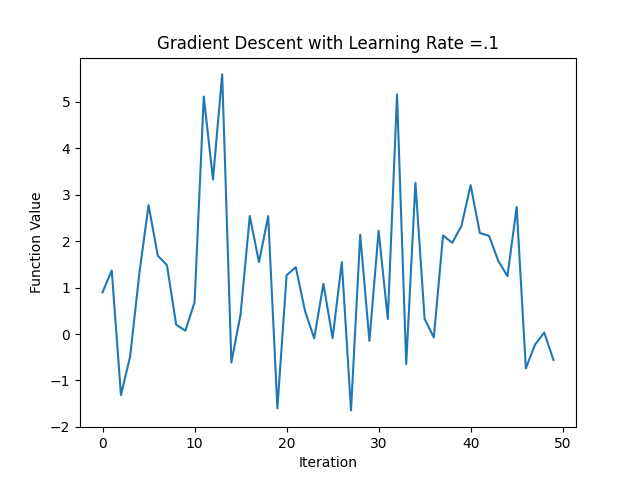
\includegraphics[width=8cm]{images/Question2/SmallRate.png} }}%
        \end{figure}
        
    \item[b. ] Table for \(\eta = .01\)
    \begin{table}[H]
        \centering
        \begin{tabular}{c|c|c}
        Initial Point & Min Location      & Min Value \\
        (.1, .1)      & (.2438, -.2379)   & -1.8201   \\
        (1,1)         & (1.2181, .7128)   & .5932     \\
        (-.5,-.5)     & (-.7314, -.2378)  & -1.3325   \\
        (-1,-1)       & (-1.2180, -.7128) & .5933    
        \end{tabular}
    \end{table}
    
    Table for \(\eta = .1\)
    \begin{table}[H]
        \begin{tabular}{c|c|c}
        Initial Point & Min Location     & Min Value \\
        (.1, .1)      & (.3484, -.0696)  & -.5591    \\
        (1,1)         & (.1985, .4578)   & .9552     \\
        (-.5,-.5)     & (-.5779, 1.4630) & 4.8314    \\
        (-1,-1)       & (-.1985, -.4578) & .9552    
        \end{tabular}
    \end{table}
\end{itemize}

\section{Problems}

\subsection{Problem 3.16} 
\begin{itemize}
    \item[a.] Given \(g(x) = P[y = +1|x]\) in the problem, then
    \begin{center}
        \(P[y = -1|x] = 1 - g(x)\)
    \end{center}
    Using this, we can solve for the expected costs:
    \begin{center}
        \(cost_{accept} = P[y = -1|x]c_a + P[y = +1|x]0\) \\
        \(cost_{accept} = (1 - g(x))c_a\)\\

        \(cost_{reject} = P[y = -1|x]0+ P[y = +1|x]c_r\) \\
        \(cost_{reject} = g(x)c_r\)
    \end{center}
    Therefore, we have shown that \(cost_{accept} = (1 - g(x))c_a\) and \(cost_{reject} = g(x)c_r\). 

    \item[b.] Assume that when \(cost(reject) \geq cost(accept)\), we accept the person. Then, we can expand to show
    \begin{center}
        \(g(x)c_r \geq (1 - g(x))c_a\) \\
        \(g(x)c_r \geq c_a - g(x)c_a\) \\
        \(g(x)c_a + g(x)c_r \geq c_a\) \\
        \(g(x)(c_a + c_r) \geq c_a\) \\
        \(g(x) \geq \frac{c_a}{(c_a + c_r)}\)
    \end{center}
    Since we know to accept if \(g(x) \geq k\) given by the problem, therefore we can conclude \(k = \frac{c_a}{(c_a + c_r)}\). 
    
    \item[c.] In Example 1.1, we are given two matrices:
    \begin{table}[H]
        \centering
        \begin{tabular}{lc|cc}
               &  & f & \\
               &  & +1 & -1 \\
            \hline
             h & +1 & 0 & 1 \\
               & -1 & 10 & 0
        \end{tabular}
        \caption{Supermarket}
        \label{tab:placeholder}
    \end{table}
    \begin{table}[H]
        \centering
        \begin{tabular}{lc|cc}
               &  & f & \\
               &  & +1 & -1 \\
            \hline
             h & +1 & 0 & 1000 \\
               & -1 & 1 & 0
        \end{tabular}
        \caption{CIA}
        \label{tab:placeholder}
    \end{table}
    The supermarket wants a low chance of false negatives, as customers may be less likely to return if their shopping experience is frustrating. This means their threshold will be low. Their \(c_a = 1\) and \(c_r = 10\), therefore, 
    \begin{center}
        \(k_{supermarket} = \frac{1}{10 + 1}\) \\
        \(k_{supermarket} \approx 0.0909 \)
    \end{center}
    The CIA wants a very low chance of false positives; employees will be willing to keep trying, and any intruders would be devastating. This means their threshold will be high. Their \(c_a = 1000\) and \(c_r = 1\), therefore, 
    \begin{center}
        \(k_{CIA} = \frac{1000}{1000 + 1}\) \\
        \(k_{CIA} \approx 0.9990 \)
    \end{center}
    
\end{itemize}

\end{document}
